% Template for a Computer Science Tripos Part II project dissertation
\documentclass[12pt,a4paper,twoside,openright]{report}
\usepackage[pdfborder={0 0 0}]{hyperref}    % turns references into hyperlinks
\usepackage[margin=25mm]{geometry}  % adjusts page layout
\usepackage{graphicx}  % allows inclusion of PDF, PNG and JPG images
\usepackage{verbatim}
\usepackage{amssymb}
\usepackage{amsmath}
\usepackage{docmute}   % only needed to allow inclusion of proposal.tex
\usepackage{listings}  % for formatting code
\usepackage{float}
\usepackage[linesnumbered,figure]{algorithm2e}
\floatstyle{boxed} 
\restylefloat{figure}

\raggedbottom                           % try to avoid widows and orphans
\sloppy
\clubpenalty1000%
\widowpenalty1000%

\renewcommand{\baselinestretch}{1.1}    % adjust line spacing to make
                                        % more readable

\begin{document}
\SetKwProg{Fn}{Function}{:}{end}

\bibliographystyle{plain}


%%%%%%%%%%%%%%%%%%%%%%%%%%%%%%%%%%%%%%%%%%%%%%%%%%%%%%%%%%%%%%%%%%%%%%%%
% Title


\pagestyle{empty}

\rightline{\LARGE \textbf{Lauren Pick}}

\vspace*{60mm}
\begin{center}
\Huge
\textbf{A Model Checker Using IC3} \\[5mm]
Computer Science Tripos -- Part II \\[5mm]
Homerton College \\[5mm]
\today  % today's date
\end{center}

%%%%%%%%%%%%%%%%%%%%%%%%%%%%%%%%%%%%%%%%%%%%%%%%%%%%%%%%%%%%%%%%%%%%%%%%%%%%%%
% Proforma, table of contents and list of figures

\pagestyle{plain}

\chapter*{Proforma}

{\large
\begin{tabular}{ll}
Name:                  & \bf Lauren Pick                           \\
College:               & \bf Homerton College                      \\
Project Title:         & \bf A Model Checker Using IC3             \\
Examination:        & \bf Computer Science Tripos -- Part II, 2016 \\
Word Count:            & \bf                                       \\
Project Originator:    & Lauren Pick                               \\
Supervisors:           & Dr Dominic Mulligan, Dr Ali Sezgin        \\ 
Supporting Supervisor: & Prof Alan Mycroft
\end{tabular}
}


\section*{Original Aims of the Project}

Describe the original aims of the project, i.e. summarize information from
the ``Substance and Structure'' and ``Success Criteria'' sections of the
project proposal.

\section*{Work Completed}

Describe the work completed as part of project, including extensions.

\section*{Special Difficulties}

None.
 
\newpage
\section*{Declaration}

I, Lauren Pick of Homerton College, being a candidate for Part II of the Computer
Science Tripos, hereby declare
that this dissertation and the work described in it are my own work,
unaided except as may be specified below, and that the dissertation
does not contain material that has already been used to any substantial
extent for a comparable purpose.

\bigskip
\leftline{Signed [signature]}

\medskip
\leftline{Date [date]}

\tableofcontents

%\listoffigures

%\newpage
%\section*{Acknowledgements}


%%%%%%%%%%%%%%%%%%%%%%%%%%%%%%%%%%%%%%%%%%%%%%%%%%%%%%%%%%%%%%%%%%%%%%%
% now for the chapters

\pagestyle{headings}

\chapter{Introduction}

%Provide a brief description of model checking in general.

Formal verification is the use of mathematics and logic to prove properties of
hardware and software systems. Formal verification techniques are
employed in several domains where the correctness of a system is
crucial, such as in hardware design and aviation.
Guaranteeing that there are no errors in hardware designs before
manufacturing begins can help avoid the high costs associated with needing to
remanufacture the hardware if the design needs to be corrected.
Additionally, the ability to prove that certain kinds of errors do not
occur are important for ensuring safety in safety-critical systems such
as those in airplanes and medical devices.

One formal verification technique is model checking.
Given a model of the system
and a specified property, a model checker will check
whether all reachable states in the system satisfy this property.
Unlike formal verification techniques that employ Hoare Logic
and theorem provers that require user guidance, model checking
is a fully automated verification technique.

In addition to being automated, because model checkers prove
properties by considering reachable states, when a model checker
discovers that a property does not hold, the model checker has
necessarily discovered a reachable state that violates the property.
A counterexample trace can, in such cases, be provided, giving
greater insight into why the property does not hold for that
model.

A brief description of symbolic model-checking and SAT-based model-checking
follows to provide further context for this project, which focuses on
implementing the IC3 algorithm, a SAT-based model-checking algorithm.


\section{Symbolic Model Checking}

%Discuss BDD-based and SAT-based model checking techniques.
All model-checking approaches suffer from limitations on the size
of the systems they can model check in practice as a result of
the state explosion problem: the number of
states in a system can be (and often is) exponential in the
number of state variables \cite{clarke12}. 

The initial approach to the model checking problem involved explicitly
considering each reachable state in the model.
Symbolic model checking arose as a method of mitigating the effects of
the state explosion problem to some extent. By representing
states and the transition relation between them as boolean
expression, symbolic model checking allows sets of states to be
represented efficiently as boolean expressions involving state variables
as opposed to an explicit list of each individual state in the set
\cite{mcmillan92}. 

Symbolic model checking was originally invented for use with ordered
binary decision diagrams (BDDs), data structures that provide an efficient
representation of boolean formulas. A unique BDD represents each logical
formula given a particular variable ordering, and an implementation that
only stores each BDD once and uses pointers appropriately can result in
less space being used.
The efficiency of BDDs in storing boolean formulas allowed for the model
checking of systems with larger numbers of states than could be handled
by explicit-state model checking \cite{mcmillan92}.

% Transition into talking about SAT-based model checking
The efficiency of BDD representations relies on choosing an appropriate
ordering, which can be computationally expensive, and in some cases,
there is no such ordering that results in a space-efficient BDD
\cite{biere99a}.

An alternative to BDD-based symbolic model-checking techniques are SAT-based
techniques, which do not use the canonical representations of boolean
formulas as BDDs and make use of procedures for solving the boolean
satisfiability problem.
Such techniques include bounded model checking (BMC),
which proves properties by finding counterexamples of certain lengths
\cite{biere99a};
$k$-induction, which proves properties inductively \cite{sheeran00};
and the IC3 algorithm that is the focus of this project.
A brief description and comparison of these techniques follows.
% Mention FSIS?
% Mention ITP?

Many modern SAT-based model checkers are based on BMC, which begins at the
initial state of the transition system and searches for paths of length
$k$ from the initial state that violate the negated property.
If no path of length $k$ is found, BMC increments $k$ and searches again.
BMC is effective at finding counterexamples, but for some large systems,
BMC is incomplete unless it is allowed to reach the point at which $k$ is
the maximal path length.

The $k$-induction algorithm is similar to BMC in its unrolling of the
transition relation to consider paths of length $k$, but it also
incorporates induction. At each depth $k$, the algorithm asserts that the
desired property holds at each state before the final state.

% Understanding IC3

\section{The IC3 Algorithm}

%Give context for the IC3/PDR algorithm, e.g. history and comparisons
%with other SAT-based model checking algorithms such as BMC and $k$-induction.

The IC3 algorithm (also called PDR \cite{een11}) is a SAT-based model-checking
algorithm for proving the safety properties (i.e. properties that must hold
in all reachable states) of hardware.
The first implementation of the algorithm \verb,ic3, placed third in
the 2010 Hardware Model Checking Competition (HWMCC'10), a competitive event
that receives model checker and benchmark submissions from industry and
academia. Its performance at HWMCC'10 generated interest in the algorithm, and
since then, several variants of the algorithm have been developed.
%2015 paper

As in $k$-induction, properties are proved through induction:
the algorithm considers reachable sets of states $k$ steps away from the
initial state until reaching a fixed point.
% Note: find when k-induction started using counterexamples
As with later variants of $k$-induction, the IC3 algorithm also discovers
new invariants if the initial assumptions are not strong enough to prove
the desired property, but unlike $k$-induction, the safety property guides
the discovery of the invariants. As a result, the discovered invariants
are more relevant for proving the safety property \cite{bradley12}.

Furthermore, IC3 does not unroll the transition relation as $k$-induction
or other BMC-based methods do, but instead considers at most one step
of the transition relation at a time, leading to smaller,
simpler SAT queries. As a result, IC3 requires less memory than BMC-based
methods in practice \cite{bradley12}.


\section{Further Work}

%Mention other applications of the IC3 algorithm, e.g. to checking
%LTL properties and to software model checking.

%Mention IIV?

While IC3 algorithm is for model checking safety properties of hardware,
there are applications of the algorithm in model checking LTL and CTL
properties and model checking software \cite{bradley12}.

The FAIR model-checking algorithm, which model checks $\omega$-regular
properties, makes use of a safety model checker such as IC3, and IICTL,
which model-checks CTL formulas \cite{hassan12}, makes use of both a
safety model checker such as IC3 as well as a fair cycle finder such as
FAIR.

Other work generalizes IC3 to use an underlying SMT solver rather than a
SAT solver, and this generalization has been used to check control-flow
graphs of programs \cite{cimatti12}.
More recently, Johannes Birgmeier, Aaron Bradley, and Georg Weissenbacher
have introduced CTIGAR, a method of abstraction-refinement based on IC3's
counterexamples to induction rather than the counterexamples in CEGAR,
which experiments suggest is competitive with CEGAR-based techniques for
software verification \cite{birgmeier14}.

\section{Project Aims}

This project's main aim is to implement a basic form of the IC3 algorithm in
Haskell that should be able to correctly check several
small examples. Additionally, the project is meant to give me an opportunity
to learn and use Haskell, to understand formal methods and especially model
checking more deeply, and to put into practice software engineering techniques.

I have successfully implemented not only a basic form of the IC3 algorithm,
which can correctly check several examples from the hardware model checking
competition in addition to the small hardware models I initially set out
to check, but also several variants of the algorithm.

\chapter{Preparation}

\section{Requirements Analysis}

%Describe the requirements for the project: AIGER parser, Minisat interface,
%transition system representation, algorithm implementation.

The model checker requires a way of taking input models and also
requires a way to solve SAT queries.
I chose the AIGER format for representing the hardware models and the
MiniSat SAT solver for answering SAT queries, resulting in a need for an
AIGER parser and a Haskell interface to MiniSat. The choice of
the AIGER format allows the model checker to be run on examples from
the Hardware Model Checking Competition, since this is the format used
to specify examples in the competitions. I chose the MiniSat SAT
solver because it is the SAT solver used by Aaron Bradley's reference
implementation of IC3 that this implementation is to be compared against.

Given that the model checking algorithm deals with transition systems
(discussed later), the implementation also requires a representation of
transition systems, which should correspond to the input hardware model.
A further requirement is the implementation of the
IC3 algorithm itself.

The main required components are thus the AIGER parser, MiniSat interface,
transition system representation, and IC3 algorithm implementation.

\section{Tools Used}

I used a variety of tools to employ software engineering practices, such
as version control and testing, and to otherwise ease the development of
the project's code.

\paragraph{Git}{
The Git version control system was used for managing the project's code. The
previous versions maintained by the version control system proved useful in
the development of the code, and branching and merging capabilities were
useful for working on and organizing different variations of the model checker.
Git submodules, which allow the inclusion of other Git projects within another
project, were used to include MiniSat within the project, enabling easier
acquisition of project dependencies (i.e., MiniSat can be obtained by running
\verb,git submodule init, after running \verb,git clone, to clone the repository).

GitHub, a widely-used hosting service for Git repositories, was used to keep
backups of the code.}

\paragraph{Haddock}{
The Haddock documentation tool for Haskell was used to generate documentation
for the code. Haddock automatically generates documentation in
several formats (e.g. HTML) from annotated Haskell code. It is commonly
used to document Haskell code, being used for most packages available
on Hackage.
}

\paragraph{HUnit}{
HUnit is a framework for writing unit tests in Haskell based on the JUnit framework
for unit testing in Java. HUnit allows tests to be specified by using functions
that return the \verb,Assertion, type to write \verb,TestCase,s. For example, the
\verb,assertBool :: String -> Bool -> Assertion, function takes a \verb,String,
that gives an error message and a \verb,Bool, value, and raises an exception (with
the error message) if the \verb,Bool, is not \verb,True,, so the following
expression would give a \verb,TestCase, that tests that function
\verb,isEven, returns \verb,True, when called with parameter 12:
\begin{verbatim}
TestCase (assertBool "Error: (isEven 12) results in False" (isEven 12))
\end{verbatim}
\begin{figure}[h]
\centering
\begin{verbatim}
data Test = TestCase Assertion
          | TestList [Test]
          | TestLabel String Test
\end{verbatim}
\caption{The HUnit {\tt Test} datatype}
\end{figure}

The \verb,Test, datatype in HUnit allows \verb,Test,s to be grouped
and built up hierarchically. Tests that have been assembled into a
singly tree can then be treated as a test suite, and the whole tree
of unit tests can be run.}

\paragraph{Criterion}{
Criterion is a library for performing benchmarking in Haskell.
Criterion can output benchmarking results in any format specified in the \verb,.tpl,
template format, and by default outputs to HTML.
The \verb,.tpl, file can be configured such that
Criterion will, for example, output benchmark sample results to a CSV, as the
\verb,.tpl, for benchmarking this project was configured.}

\paragraph{Cabal}{
Cabal is the standard package and dependency management system for Haskell,
where a package may be either a library or a complete piece of software.
Information about a Cabal package, such as its version and dependencies,
is specified through a \verb,.cabal, file in its root directory.
The \verb,.cabal, file may contain several different sections, such as a
\verb,library, section, describing the modules in the package that should be
exposed in the library provided by the package or an \verb,executable, section,
which has fields for specifying the Haskell file containing the \verb,Main,
module and for specifying other Haskell files used by the program.
The \verb,.cabal, file for this project also uses the \verb,Test-Suite, section
to allow the HUnit test for the project to be run in a standard way (by running
\verb,cabal test, in the root directory of the package) and the \verb,Benchmark,
section to allow the benchmarking program to be run in a standard way also
(by running \verb,cabal bench, in the root directory of the package).

Cabal also uses a Haskell file \verb,Setup.hs, to give further information
about how to build the package. For example, the \verb,Setup.hs, file
for this project compiles the C and C++ code needed for the project before
Cabal attempts to build the rest of the project, so the files necessary
for linking are already present.

The use of Cabal enables the project to be built easily on different platforms,
since Cabal provides a standard method for building the package that works
across platforms.}

\paragraph{hsc2hs}{
The \verb,hsc2hs, preprocessor eases the writing of Haskell bindings to C
code by enabling the programmer to write a \verb,.hsc, file containing
macros that the preprocessor can expand to, e.g., pointer offsets. The
\verb,hsc2hs, expands the macros in a \verb,.hsc, file to produce a
\verb,.hs, file that can then be compiled with a Haskell compiler and run.
}

\paragraph{Aiger Utilities}{
Several tools provided in Aiger Utilities were used in the project. The
AIGER parser provided was used for comparison with and as an alternative
to the one developed as part of this project. 

The Aiger Utilities' tools to convert between formats for specifying
hardware models eased the specification of new hardware models that would
be compatible with the model checker, which accepts only AIGER-formatted inputs,
and that would be compatible with  Aaron Bradley's reference implementation of IC3,
which takes only the binary format of AIGER as input.
In particular, the tools of use were
the {\tt bliftoaig}
tool, which converts a circuit specified using the Berkeley Logic Interchange Format
to a circuit specified using the binary AIGER format, and the {\tt aigtoaig} tool,
which converts between the ASCII and binary AIGER formats.
}

\paragraph{MiniSat}{
MiniSat is a SAT solver implemented in C++ that solves boolean satisfiability problems
posed in conjunctive normal form. Further details are given in section \ref{MiniSat}.
}

\section{Symbolic Representation}
I give a brief review of concepts in logic, and introduce transition systems and the
representation of states using boolean formulas.

\paragraph{Logic}{
Unless otherwise specified, a variable is a propositional symbol,
and can be assigned to boolean values {\it True} or {\it False}.
A literal is defined as being either a variable $v$ or its negation $\neg v$.

The concepts of a cube and a clause are useful in describing the
representation of states as boolean formulas.
A cube is defined to be a conjunction of literals and may be represented as the set
of literals that occur in it. Similarly, a clause is a disjunction of literals that
may also be represented as the set of literals that occur in it. Through the
application of deMorgan's laws, the negation of a cube is a clause and vice-versa.

A boolean formula is in conjunctive normal form (CNF) if it is a conjunction 
$\bigwedge_i D_i$ of disjunctions $D_i$ of literals (i.e. clauses). A set of clauses
can and often will be interpreted as the CNF formula resulting from the conjunction
of the clauses.}

\paragraph{Transition Systems}{
A transition system is a tuple $(i,x,I,T)$ consisting of a set of input
variables $i$, state variables $x$, an initial
set of states represented by the boolean expression $I(x)$ and
a transition relation represented by the boolean expression $T(i,x,x')$,
where $x'$ is the set of next-state variables.

For each state variable $v$, $v'$ denotes the corresponding next-state variable.
For example, a transition relation that states that all variables that are
currently {\it True} should become {\it False} in the next state is as follows:
$$T(i,x,x') = \bigwedge_{v \in x} (v \Rightarrow \neg v').$$

Given transition relation $(i,x,I,T)$, a boolean formula $C$ is, by definition,
be inductive relative to another boolean formula $F$ if both
$I \Rightarrow C$ and $F \wedge C \wedge T \Rightarrow C'$ hold.
}

\paragraph{States}{
A single state of the transition system (or a singleton set containing that state)
is specified through the assignment of all variables in the transition system
to boolean values, where a complete assignment is represented as a cube such
that every variable appears in the formula exactly once.
An incomplete assignment of variables in the transition system is a cube such that
at least one variable in the transition system does not appear in the cube. Such an
assignment $c$ specifies the set of cubes $\{a \in{\it Full~Assignment}|c \subset a\}$,
where ${\it Full Assignment}$ is the set of complete assignments to the variables in the
transition system.
More generally, any boolean expression $b$ involving the variables in the transition
system gives the set of states
$\{a \in {\it Full~Assignment} | a \wedge b~{\rm is~satisfiable}\}$.

A state that is in the set of states represented by a boolean formula $B$ is referred to
as a $B$ state. A set of states $s$ is said to be reachable
in $k$ steps of the transition relation iff there exist states $s_0, \ldots, s_k$ such that
$s_0$ is an $I$ state and $s_i \wedge T \Rightarrow s_{i + 1}$ for $1 \leq i < k$.

}


\section{Model Specification}
%Describe the AIGER (old and new version) and BLIF formats and
%{\tt bliftoaig} from the AIGER utilities.

%Comments?

I used both the AIGER format and Berkeley Logic Interchange Format (BLIF)
to specify the example hardware models that were not taken from the
Hardware Model Checking Competition.
The hardware models that the model checker accepts as input
are specified using the AIGER format;
however using the AIGER format to specify larger models was cumbersome,
so such models were specified using BLIF and converted to AIGER format
using the Aiger Utilities' \verb,bliftoaig, tool.

Inputs to model checker are models formatted using either the ASCII or
binary AIGER formats described below.

The AIGER format provides a method of specifying hardware modeled as
And-Inverter Graphs with latch elements providing single clock-tick
delays: all circuits are modeled as a graph of nodes consisting only of
AND gates, inverters, and latches.

The AIGER format has both an ASCII and a binary version. The ASCII
format is more flexible and human readable, imposing fewer constraints
on the ordering of components within the input file. For example, an
AND gate with variable name 20 may be specified before an AND gate with
variable name 11 in the ASCII format, but AND gates must be specified in
ascending order of their variable names in the binary AIGER format. Another
example is that AND gates' inputs can be specified in any order in the ASCII
format, but the binary format encodes AND gates under the assumption
that inputs are specified in ascending order.
The the binary version's assumptions on component ordering allows the format
to be more compact. The Hardware Model Checking Competition's examples
use the binary format.

A new version of the AIGER format is currently under development, with
examples from HWMCC'14 using the new version. The AIGER parser implemented
as part of this project handles both the old and new versions of the AIGER
format.

\paragraph{AIGER Variables}{
A variable's name in AIGER format is a positive integer. Variables themselves
are not represented directly in AIGER format; instead, nonnegative numbers
are used to represent literals and boolean valies.
I will refer to these nonnegative numbers as indices.

For any variable named $x$, the index for positive literal $x$ is given by
$2 \times x$, and the index for negative literals $\neg x$ is given by
$2 \times x + 1$, i.e. a function to map from variable names $x$ and a boolean
value $b$ giving the sign of the literal would be as follows:
$${\it index}(x, b) =
\begin{cases}
2x & {\rm if}~b \\
2x + 1 & {\rm otherwise}
\end{cases}$$
The indices 0 and 1 are used to represent the constant boolean values {\it False}
and {\it True}, respectively.

It is apparent that any index above 1 represents a literal and that for all such
indices, all even indices represent positive literals, and all odd indices
represent negative literals. The representation thus allows an implementation
use the least significant bit of an index to be used to find the sign of a literal,
and a single bitwise right shift to find the variable name for the literal.

\paragraph{Old version}{
All AIGER files in the old version begin with a header of the form
\begin{verbatim}
V M I L O A
\end{verbatim}
where
\begin{itemize}
\item \verb,V, can take on values \verb,aag,, specifying that the file is in the ASCII format or \verb,aig,,
specifying that the file is in the binary format.
\item \verb,M, gives the maximum index of a variable.
\item \verb,L, gives the number of latches.
\item \verb,O, gives the number of outputs.
\item \verb,A, gives the number of two-input AND gates.
\end{itemize}

The different components are specified after the header
in the order that their counts are given in the header.

In the ASCII version of the format, inputs are specified by giving the
index that represents the positive literal for its corresponding variable name,
and outputs are specified similarly as single indices (that may represent
booleans or literals of any sign).

Latches have initial value 0 (i.e., {\it False}) and are specified by giving the
index representing the positive literals for their corresponding variable name
followed by the index for their next-state value.
AND gates are specified by giving the indices that represent the positive literal
for their variable name and the two indices that specify their input values.

\begin{figure}[h]
\centering
\begin{verbatim}
aag 3 0 2 1 1
2 3
4 2
6
6 2 4
\end{verbatim}
\caption{
A circuit specified in the old ASCII AIGER format
}
\label{aagCircuit}
\end{figure}

\begin{figure}[h]
\centering
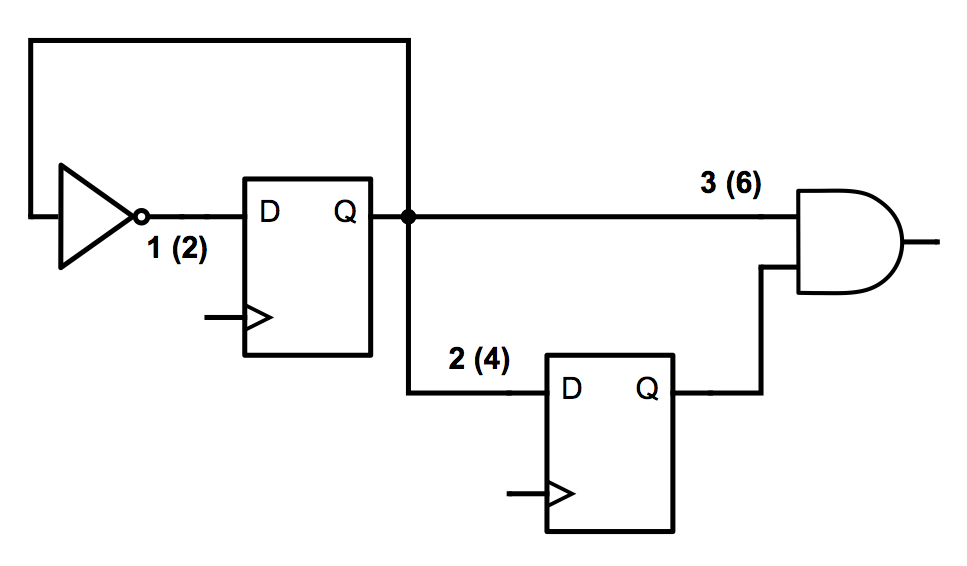
\includegraphics[width=100mm]{circuit.png}
\caption{The circuit represented by figure \ref{aagCircuit}, where
the variable name for each component is directly to the left of that
component, with the corresponding index in parenthesis.}
\end{figure}

For example, figure \ref{aagCircuit} specifies a circuit with
no inputs, two latches with indices $2$ and $4$ and one AND gate
$6$ that takes the outputs of the two latches as inputs and whose
output is the single output of the circuit.}

\paragraph{Binary version}{
In the binary version of the format, variable indices are assumed to
occur in increasing order. Since each literal must be defined, this allows
for the omission of the variable indices when defining inputs or latches.

Inputs are not explicitly listed: the input variables are inferred based on
the value of \verb,I,.
Similarly, latches are specified by only listing their next-state literals'
representations.

The binary format also assumes that AND gates occur in order of their
variable indices and additionally assumes that inputs to an AND gate will
have already been defined before that AND gate.
These assumptions allow AND gates to be represented by two differences
that tend to be small in practice:

For an AND gate specified in the old format by \verb,lhs rhs0 rhs1,,
where inputs \verb,rhs0, and \verb,rhs1, have been ordered such that
$\verb,rhs0, \geq \verb,rhs1,$, define
$$\delta_0 = \verb,lhs, - \verb,rhs0,$$
and
$$\delta_1 = \verb,lhs, - \verb,rhs1,$$

The values $\delta_i$ are then represented with the following binary
encoding, giving a more compact representation for AND gates than
the ASCII version of the format:

For 7-bit words $w_0, \ldots w_n$ with
$$\delta_i = w_0 + 2^7w_1 + \ldots + 2^{7n}w_n,$$
$\delta_i$ is represented as the sequence of $n + 1$ bytes
$b_0, \ldots, b_n$, where
\begin{itemize}
\item for $0 \leq k < n$, $b_k$ is the byte obtained by setting the most
significant bit to 1 and the rest of the bits to $w_k$, and
\item $b_n$ is the byte obtained by setting the most
significant bit to 0 and the rest of the bits to $w_n$
\end{itemize}}


\paragraph{New version} {
The new AIGER format begins with a header of the form
\begin{verbatim}
V M I L O A B C J F
\end{verbatim}
where \verb,V,, \verb,M,, \verb,I,, \verb,L,, \verb,O,, \verb,A, are as
in the old format, and
\begin{itemize}
\item \verb,B, gives the number of ``bad state'' properties
\item \verb,C, gives the number of invariant constraints
\item \verb,J, gives the number of justice properties
\item \verb,F, gives the number of fairness constraints
\end{itemize}

Components are specified after the header in the same order that their
counts are given in the header with the exception of AND gates, which
occur at the end of the file. Latches' initial values can also be specified
now with an additional \verb,0, or \verb,1, after the next-state literal's
index. If the initial value is omitted, the initial value is assumed to be
0 as in the old version of the format. The header can also be truncated
after giving the number of AND-gates if the remaining counts are all
zero, allowing any parser for the new AIGER format to be
backwards-compatible.

The new version of the format is otherwise
the same as the old format.}

\section{The IC3 Algorithm}
%Describe how the IC3 algorithm works when trying to prove a model has a property
%$P$.
Given a hardware model (i.e. a finite-state transition system $(i,x,I,T)$) and a
safety property $P$, IC3 aims either to prove inductively that $P$ holds
at all reachable states from the initial state or
to find a $\neg P$ state that can be reached.
The following pseudocode gives an overview of the basic IC3 algorithm:

\begin{algorithm}[H]
\DontPrintSemicolon
\Fn{prove$((i,x,I,T),P)$}{
  \lIf{$\neg (I \Rightarrow P)$ \label{initiation}}{
    \Return{False}
  }
  $F_0 := I$ \;
  $k := 0$ \;
  \While{True \label{main}}{
    \eIf{$F_k \wedge T \Rightarrow P'$ \label{consecution}}
    {create frame $F_{k + 1}$ initialized to $\emptyset$\;
     $k$ := $k + 1$ \;}
    {\While {$\neg (F_k \wedge T \Rightarrow P')$ \label{reconsec}}{
        ${\it cti} := {\it nextCTI}(F_k \wedge T \Rightarrow P')$ \label{CTI} \;
        \lIf{{\it proveNegCTI}$((i,x,I,T),{\it cti},k - 1)$ \label{negCTI}}{$F_k$ := $F_k \cup \{\neg{\it cti}\}$}
        \lElse{\Return{False}}}} \label{Unsafe}
    \For{ i = 0 \KwTo $k - 1$ }{ \label{forprop}
      $F_{i + 1} := F_{i + 1} \cup \{c \in F_i | F_i \wedge T \Rightarrow c'\}$ \label{push} \;
      \lIf {$F_i = F_{i + 1}$}{\Return {True}} \label{fixed}
    }
  }
}
\caption{An overview of the IC3 algorithm. Frames are assumed to be passed by reference:.}
\label{overview}
\end{algorithm}

The IC3 algorithm maintains a set of $k + 1$ frames $F_0,\ldots,F_k$, where
each frame $F_i$ is a set of clauses whose disjunction represents an
overapproximation of the set of states that reachable by the transition
system in at most $i$ steps
(so, for example, $F_0$ is just the initial state set $I$, as seen
in the pseudocode).
The deepest frame $F_k$ in the set of frames is called the frontier frame.

%Initiation query
The initiation query $I \Rightarrow P$ on line \ref{initiation} is used to check that the safety
property holds in the initial state $I$.
This query is run once at the start of
the algorithm for the desired safety property.
If it fails (i.e. if it is {\it False}), then the algorithm terminates,
as an error state in which $\neg P$ holds is reachable in 0 steps.
If the query succeeds, then the algorithm proceeds to its main loop.

The main loop of the algorithm is the while-loop beginning on line \ref{main}.
The algorithm only exits the loop when it has determined whether or not the
safety property holds at all reachable states in the model.

%Consecution query
The consecution query $F_k \wedge T \Rightarrow P'$ on line \ref{consecution} is
is used to check whether the property $P$ necessarily holds in the next
frame. If it succeeds (i.e., if it is {\it True}), then IC3 creates a new
frontier frame $F_{k + 1}$.
%Describe what happens when a consecution query fails
If a consecution query $F_k \wedge T \Rightarrow P'$ fails, then that means that
there is an $F_k$ state that is a predecessor of the $\neg P'$ state,
i.e. there is an $F_k$ state $s$ and a $\neg P'$ state $v$ with $T(i,s,v')$.
The state $s$ is called a \emph{counterexample to induction} (CTI) state.

The algorithm aims to refine the approximation $F_k$ of the set of states
reachable in at most $k$ steps by showing that all states that are
reachable in at most $k$ steps are $\neg s$ states.

The call to {\it nextCTI} in line \ref{CTI} finds the counterexample to
induction state $s$. The call to {\it proveNegCTI} on line \ref{negCTI}
attempts to prove that $\neg s$ is inductive relative to $F_{k - 1}$,
so that all $F_k$ states are necessarily $\neg s$ states, so $\neg s$ can
be added to the set of $F_k$ clauses.

The {\it proveNegCTI} function works similarly to the
while loop on line \ref{reconsec}. For as long as the query
$F_k \wedge \neg s \wedge T \Rightarrow s'$ is unsuccessful,
the algorithm extracts a counterexample to induction cube and
calls {\it proveNegCTI} to show that the counterexample is
inductive relative to frame $F_{j - 1}$ so that the negated
counterexample can be added to frame $F_j$.
If the shallowest possible depth $j = 0$ is reached, then
{\it proveNegCTI} fails and returns {\it False}.

The {\it proveNegCTI} pseudocode does not explicitly check for $I \Rightarrow
\neg s$. An explicit check is unnecessary because if
$I \Rightarrow \neg s$ does not hold, then eventually ${\it proveNegCTI}$
will be called recursively with $j = 0$ and the attempt to show that
$\neg s$ is relatively inductive to $F_j$ fails.

\begin{algorithm}[H]
\DontPrintSemicolon
\Fn{proveNegCTI$((i,x,I,T),s,j)$}{
  \lIf{$j = 0$}{\Return{False}}
  \While{$\neg(F_j \wedge \neg s \wedge T \Rightarrow \neg s')$}{
    ${\it cti} := {\it nextCTI}(F_j \wedge \neg s \wedge T \Rightarrow \neg s')$ \;
    \lIf{{\it proveNegCTI}$((i,x,I,T),{\rm cti},j - 1))$}{$F_j$ := $F_j \cup \{\neg{\it cti}\}$}
    \lElse{\Return{False}}
  }
}
\end{algorithm}

If $\neg c$ cannot be proven to hold at $k$ steps of
the transition relation from the initial state, i.e. the state $s$ is in the actual
set of states reachable in $k$ steps from the initial state, then a $\neg P$ state
is reachable in $k + 1$ steps from the initial state; the safety property does not
hold, and the algorithm terminates (line \ref{Unsafe}).

Because there may be several counterexamples to induction, it is necessary to
perform the consecution query again (line \ref{reconsec}). If it fails again,
the process of finding the new counterexample to induction state(s) $d$ and trying to
prove that $\neg d$ holds at depth $k$ repeats. Upon the success of the consecution
query, the algorithm moves to the propagation phase.

Pushing a clause $c$ from a frame $F_i$ to frame $F_{i + 1}$ refers to the act
of setting $F_{i + 1} := F_{i + 1} \cup \{ c \}$.
A clause $c$ can be pushed from a frame $F_i$ to the next frame $F_{i + 1}$
if the consecution query $F_i \wedge T \Rightarrow c'$ holds.
The propagation phase of the algorithm goes through the set of frames
$F_0, \ldots, F_k$, and, for every $F_i$ with $0 \leq i < k$ (line \ref{forprop}),
pushes all the clauses that it can from $F_i$ to $F_{i + 1}$ (line \ref{push}).

If $F_i = F_{i + 1}$ holds for any $i$ at any point, then a fixed point has
been found: frames at any greater depth than $i$ will continue to be the
same as $F_i$, since all the the clauses in $F_i$ and therefore $F_{i + 1}$
can be pushed.
Because $F_i$ contains the safety property $P$ as one of its clauses,
this means that $P$ holds in all reachable states from the initial state,
and the algorithm terminates (line \ref{fixed}).

\subsection{Generalization}

After showing that a negated CTI state $\neg s$ is relatively inductive to a
frame $F_i$ and adding the clause $\neg s$ to frame $F_{i + 1}$, the state
$s$ is eliminated from the approximation $F_{i + 1}$ of the set of states
reachable in at most $i + 1$ steps. An improvement can be made by generalizing
$s$ to a set of several states $c$ rather than a single state, and treating
$c$ as the CTI. If $\neg c$ is successfully proven to be relatively inductive
to $F_i$, then adding it to frame $F_{i + 1}$ eliminates several states (i.e.,
all $c$ states) at once rather than only $s$. Because the cube $c$
is chosen so that $\neg c \Longrightarrow \neg s$, at least one CTI state
has been removed from $F_{i + 1}$, and because $c$ contains several states,
it is possible that several CTIs may have been removed from $F_{i + 1}$
by adding the clause $\neg c$ to it. The process of finding such a cube $c$
is referred to as \emph{generalization}.

\subsection{Minimal Inductive Subclauses}
The \emph{minimal inductive subclause} for a frame $F_i$ and a clause $\neg s$ that
is inductive relative to $F_i$
(i.e. $F_0 \Rightarrow s'$ and $F_i \wedge T \wedge s \Rightarrow s'$)
is a clause $\neg c$ whose
literals are the smallest subset of the literals in $\neg s$ such that
$\neg c$ is also inductive relative to $F_i$.

The minimal inductive subclause can be found by dropping each literal
in $s$ in turn and checking if the resulting clause is inductive
relative to $F_k$:

\begin{algorithm}[H]
\DontPrintSemicolon
\Fn{mic(cls,k)}{
  \ForEach{literal l in cls}{
    $subcls := cls \setminus \{l\} $\;
    \If{subcls {\rm is inductive relative to frame at depth} k}{
      $cls := subcls$ \;
    }
  }
  \Return{cls} \;
}
\end{algorithm}

%Finding the minimal inductive subclause can be computationally
%expensive, so it is often approximated in practice.

A

An improvement to the generalization provided by finding minimal
inductive subclauses in this way incorporates the use of counterexamples
to generalization.

\subsubsection{Counterexamples to Generalization}

Checking if a subclause $\neg c = s \setminus \{l\}$ of a clause $\neg s$ is inductive
relative to a frame $F_i$, involves checking if
$F_i \wedge T \wedge \neg c \Rightarrow \neg c'$ holds.
If the implication does not hold, then $\neg c$ is not inductive relative to
$F_k$. In the original method of generalization described above,
this means that $\neg s$ cannot be generalized to $\neg c$, and generalization
proceeds without dropping $l$.

It could be the case that the reason that the query
$F_k \wedge T \wedge c \Rightarrow c'$ is unsatisfiable because
$F_k$ is too broad an approximation, similarly to why a consecution
query at $F_k$ might fail. As with consecution queries, discovering a
new clause that can be added to $F_k$ may allow the queries that
check for relative induction to succeed, and the discovery of this
clause can be directed by a counterexample extracted from the
SAT-solver after the query for $F_k \wedge T \wedge c \Rightarrow c'$.

The counterexample state in this case is called a \emph{counterexample
to generalization} (CTG), and proving the negated CTG to be true at
frame $F_k$ allows $s$ to be generalized to $c$.


\chapter{Implementation}

The implementation can be broken up into four main components: the AIGER parser, the
MiniSat interface, the hardware model representation, and the model checker.


\section{Parser}
%Discuss the implementation of the AIGER parser. In particular, mention
%the handling of both the older and newer AIGER format versions for both
%the ASCII and binary versions of the format and the representation
%of AIG models.

The parser component parses both ASCII or binary-formatted AIGER files and
assumes that the new format is used (because all old format AIGER files are also
new instances of the new format). The justice properties and fairness constraints
are ignored by the parser, as they are not used by the model checker.

Both the \verb,Parser.AigerParser, module that implements the parser in Haskell and
the \verb,Parser.AigerTools, module that calls the Aiger Utilities' parser's functions
parse the AIGER file into the \verb,Model, data structure in \verb,Parser.AigModel,,
which stores the components specified in the AIGER file.

\subsection{Model}

More specifically, the \verb,Model, data structure stores the number of variables and
the number of inputs. It also stores as a list of literals the outputs, bad states,
and invariant constraints. The data structure also stores latches and AND gates as
lists of lists of literals. I discuss the representation of literals, latches, and
AND gates below.

Literals are represented by a \verb,Lit, data structure in the \verb,Parser.AigModel,
module, which stores decoded versions of AIGER format indices:
The \verb,Lit, data structure has a constructor \verb,Boolean, that takes a \verb,Bool,
argument for representing the boolean values that correspond with AIGER indices
0 and 1, a \verb,Var, constructor that takes a \verb,Word, for representing a positive literal,
and a \verb,Neg, constructor that takes a \verb,Word, for representing a negative literal.
Variable names are adjusted (by subtracting 1) so that they start at 0.

\begin{figure}[H]
\centering
\begin{verbatim}
data Lit = Var Word | Neg Word | Boolean Bool
\end{verbatim}
\caption{The {\tt Lit} data structure in {\it Parser.AigModel}}
\end{figure}

For example, the index 3 read from an AIGER file is parsed into \verb,Neg 0,:
the odd index 3 indicates that it is a negative literal of the variable named 1, and
subtracting by 1 gives the new variable name 0.

Latches and AND gates are represented using three-element \verb,Lit, lists.
For latches, the first element gives the variable name of the latch (as a positive literal),
the second gives the next-state literal, and the final element gives the initial state
of the latch. For AND gates, the first element gives the variable name of the AND gate
(as a positive literal), and the next two elements give the literals whose values are taken
as inputs to the AND gate.

\section{MiniSat Interface}
%Describe the process of implementing the Haskell bindings for Minisat
%functions, including the wrapper functions for Minisat written in C.

MiniSat serves as the SAT solver for this implementation of the IC3 algorithm.
Because the Haskell Foreign Function Interface cannot interface with C++ directly,
the interface to the MiniSat SAT solver is composed of a C wrapper for the relevant
MiniSat functions and classes and a Haskell interface to the C wrapper.

\subsection{MiniSat Overview}
\label{MiniSat}

To solve a SAT query, MiniSat creates an instance of a \verb,Solver, object,
which contains a set of variables, sets of clauses, and possibly a model or a conflict vector.
The set of variables in the \verb,Solver, gives all the variables that may appear in
a SAT query, the set of clauses forms the SAT query, and the model or conflict vector
gives further information about the last SAT query made.

In addition to a \verb,Var, type for representing variables, MiniSat has a \verb,Lit, type for
representing literals, and MiniSat represents sets of clauses as \verb,vec<Lit>,s,
vectors of literals. The set of clauses in a \verb,Solver, together represent a CNF query,
so that if the \verb,Solver,'s \verb,solve(), function is called,
the resulting \verb,bool, indicates whether the query is satisfiable or not. The
\verb,solve(), function is overloaded so that it may also take an assumption \verb,vec<Lit>*, as
an argument. The literals in the assumption vector must hold in addition to the CNF query formed
by the \verb,Solver,'s clauses: if the \verb,Solver,'s clauses form some CNF query $C$ and
\verb,solve(assumps), is called, where \verb,assumps, points to the the assumption vector
containing all the literals in some set $A$, then the SAT query is $C \wedge \bigwedge_{l \in A} l$.

If at least one query to a \verb,Solver, has been made, then if the last query to the
\verb,Solver, was satisfiable, the \verb Solver, provides a \verb,model, pointer
to a set of satisfying variable assignments for that query, or, if the last query to the solver
was not satisfiable, the \verb,conflict, pointer to a set of literals from the assumption
vector provided in the query that contributed to the query being unsatisfiable.

If there has been at least one query made of the \verb,Solver, object, and the query was
satisfiable, the \verb,Solver,'s \verb,model, variable points to a set of variable assignments
for that SAT query.
If there has been at least one query made of the \verb,Solver, object, and the query was
unsatisfiable, the \verb,Solver,'s \verb,conflict, variable points to a set of literals that
contains the assumed literals that caused the query to be unsatisfiable.

This model checker uses instances of \verb,SimpSolver,, a subclass of the \verb,Solver, class
that does simplification and returns full assignments.

\subsection{C Wrapper}

Much of the C wrapper is straightforwardly as follows: every MiniSat class is replaced with a C
type, and every MiniSat function is replaced with a function with an \verb,extern C, function that
calls the MiniSat C++ function, as in figure \ref{addClause}.

\begin{figure}[h]
\begin{verbatim}
extern "C" int addMinisatClause (Minisat::SimpSolver* solver,
                                 Minisat::vec<Minisat::Lit>* ps) {
  return solver -> addClause (*ps);
}
\end{verbatim}
\caption{The C wrapper function for {\tt addClause} from {\tt CSolver.cpp}}
\label{addClause}
\end{figure}

I also added an additional \verb,result, struct to allow for all the results of a SAT query to
be returned from a single function call. The struct contains not only the result of the SAT
query, but also pointers to the model and conflict vector (if any) of the \verb,Solver,.
The wrapper function \verb,solveWithAssumps, for the version of \verb,solve(), that takes an assumption
vector as an argument and returns a pointer to a \verb,result, struct
rather than just whether or not the query was satisfiable.

\begin{figure}[h]
\begin{verbatim}
struct result {
  unsigned solved;
  unsigned modelSize;
  unsigned conflictSize;
  minisatLbool* model;
  litptr* conflict;
} res = {0, 0, 0, 0, 0};
\end{verbatim}
\caption{The {\tt result} struct from {\tt CSolver.h}}
\end{figure}

\subsection{Haskell Interface}

The Haskell interface makes use of the Haskell FFI as well as the \verb,hsc2hs, preprocessor
for handling the \verb,result, struct.

Using just the Haskell FFI for calling the C functions does not provide a
sufficient abstraction for use by the rest of the model checker.
I wrote further functions to allow for a more natural interface to MiniSat,
 making use of \verb,unsafePerformIO, to have the functions return
values outside the \verb,IO, monad.

Many of the functions and datatypes in the interface are analogous to functions and structs in
the C wrapper and C++ implementation of MiniSat. For example, the \verb,Solver, datatype is an
analogue to the MiniSat \verb,Solver, object, and itself contains a pointer to an instance of
a MiniSat \verb,Solver, object. Similarly, functions such as \verb,solveWithAssumps, work
analogously to the C wrapper's \verb,solveWithAssumps,, returning a \verb,Result, that contains
whether or not the query was satisfiable and the model or conflict vector (if any).

The information kept in a \verb,Result, is taken directly from the \verb,result, returned by
the C Wrapper functions. I used the \verb,hsc2hs, preprocessor to help handle pointer offsets
when unmarshalling from the C struct. Beyond straightforward unmarshalling, some additional work
to convert from the MiniSat representation of literals to the model checker’s representation of
literals was necessary.

\section{Hardware Models}
\subsection{Representation}
\subsubsection{Literals}
The \verb,Lit, data structure in \verb,Model.Model, gives the representation for literals in
the model checker.
The \verb,Var, constructor gives positive current-state (unprimed) literals, the \verb,Neg,
constructor gives negative current-state literals, and the \verb,Var', and \verb,Neg', constructors
respectively give positive and negative next-state (primed) literals.

\subsubsection{Transition Systems and Safety Properties}
% Describe how transition systems and safety properties are represented.
The representation of transition systems and the safety property for the model checker to check
are both encompassed in the \verb,Model, data structure in \verb,Model.Model,, which serves
as the representation of the hardware in the model checker.
The inputs $i$ and state variables $x$ in the transition system $T(i,x,I,T)$
are not distinguished, and the total count of variables is kept in \verb,vars,.
Clauses that specify the initial state $I$ are kept in \verb,initial,.
The transition relation $T$ is captured by \verb,transition,, a list of both clauses that specify
latches and clauses that specify AND gates.
The literal that gives the safety property is given by \verb,safe,.

\begin{figure}[H]
\centering
\begin{verbatim}
data Model = Model { vars :: Word
                   , initial :: [Clause]
                   , transition :: [Clause]
                   , safe :: Lit } deriving Show
\end{verbatim}
\caption{The data structure for representing the hardware model in the model checker.}
\end{figure}

\subsection{Construction}
% Describe how transition systems are constructed given AIG models.

The \verb,Model.Model, module contains functions to convert the \verb,Model, data
structure in \verb,Parser.AigModel, into the hardware model representation used by
the model checker. In particular, the \verb,toModel, function takes an \verb,Parser.AigModel.Model,
and outputs a \verb,Model.Model.Model,. The \verb,Model.Model, module has its own \verb,Lit,
data structure that only has constructors for positive and negative literals; \verb,Lit,s from
the \verb,Parser.AigModel, module are either converted to \verb,Model.Model.Lit,s or, in the case
that they use the \verb,Boolean, constructor, are removed from the model during the conversion of
the \verb,Latch, and \verb,And, components to \verb,Clause,s in \verb,Model.Model,.

The \verb,makeLatches, function generates a pair of \verb,Clause, lists
for a list of \verb,Parser.AigModel.Latch,es, where the first \verb,Clause, list contains
clauses that describe the latches' initial values, and the second \verb,Clause, list
contains a clauses that describe the latches' next-state values. For a given
\verb,Parser.AigModel.Latch, \verb.[latchVar, next, init]., if \verb,init, is \verb,Boolean True,,
then the singleton clause containing only the positive literal for \verb,latchVar, is generated for
the initial value list, and if \verb,init, is \verb,Boolean False, then the negative literal for \verb,latchVar,
is generated.
Similarly, if \verb,next, is \verb,Boolean True,, then the singleton clause containing only the positive primed
literal for \verb,latchVar, is generated for the next-state list because the next-state value for the variable
is a constant-{\it True} value, and similarly, if \verb,next, is \verb,Boolean False,,
the singleton clause containing only the negative primed literal for \verb,latchVar, is generated.
Otherwise, the next-value clauses generated for \verb,latchVar, are $\{\verb,latchVar',, \neg \verb,next,\}$
and $\{\neg\verb,latchVar',, \verb,next,\}$. The conjunction of these clauses are, as needed, logically equivalent
to ${\tt next} \Longrightarrow {\tt latchVar}'$, i.e., where $\simeq$ denotes logical equivalence,
the following hold:
\begin{align*}
{\tt latchVar}' \Longleftrightarrow {\tt next} &\simeq ({\tt latchVar}' \Longrightarrow {\tt next}) \wedge
({\tt next} \Longrightarrow {\tt latchVar}')\\
{\tt latchVar}' \Longrightarrow {\tt next} &\simeq \neg {\tt latchVar}' \vee {\tt next}\\
{\tt next} \Longrightarrow {\tt latchVar}' &\simeq {\tt latchVar}' \vee \neg {\tt next}.
\end{align*}
It follows that the original double implication is equivalent to the 
the CNF formula that corresponds to the generated clauses:
$${\tt latchVar}' \Longrightarrow {\tt next} \simeq
(\neg {\tt latchVar}' \vee {\tt next}) \wedge ({\tt latchVar}' \vee \neg {\tt next}).$$

The \verb,makeAnds, function generates a single \verb,Clausse, list for a list of \verb,Parser.AigModel.And,s,
where for each \verb,And,, of the form \verb.[andVar, in1, in2]., if both \verb,in1, and \verb,in2, use
the \verb,Boolean, constructor for \verb,Parser.AigModel.Lit,s, then \verb,makeAnds, generates a singleton
clause containing the positive unprimed variable for \verb,andVar, if both \verb,in1, and \verb,in2, are
\verb,Boolean True,, since theit conjunction gives a constant-{\it True} value for the current state of
\verb,andVar, and generates a singleton clause containing the negative unprimed variable for \verb,andVar,
otherwise, since if either input to an AND gate is {\it False}, the output of the AND gate is also {\it False}.
If only one of \verb,in1, or \verb,in2, is a \verb,Boolean,, then if it is \verb,Boolean False, clauses equivalent
to ${\tt makeAnds} \Longleftrightarrow {\it in}$, where ${\it in}$ is the non-\verb,Boolean, variable
are generated using the logical equivalence employed in generating the \verb,Latch, next-state clauses, i.e.
the clauses $\{\verb,andVar,, \neg {\it in}\}$ and $\{\neg\verb,andVar,, {\it in}\}$ are generated.
If neither of \verb,in1, or \verb,in2, are \verb,Boolean,s, then the clauses generated are
$\{\neg\verb,andVar,, \verb,in1,\}$, $\{\neg\verb,andVar,, \verb,in1,\}$, and
$\{\neg\verb,in1,,\neg\verb,in2,,\verb,andVar,\}$. The conjunction of these clauses are, as needed,
logically equivalent to $\verb,andVar, \Longleftrightarrow \verb,in1, \wedge \verb,in2,$:
\begin{align*}
{\tt andVar} \Longleftrightarrow {\tt in1} \wedge {\tt in2} &\simeq
({\tt andVar} \Longrightarrow {\tt in1} \wedge {\tt in2}) \wedge
({\tt in1} \wedge {\tt in2} \Longrightarrow {\tt andVar})\\
{\tt andVar} \Longrightarrow {\tt in1} \wedge {\tt in2} &\simeq
\neg {\tt andVar} \vee ({\tt in1} \wedge {\tt in2})\\
{\tt in1} \wedge {\tt in2} \Longrightarrow {\tt andVar} &\simeq
\neg ({\tt in1} \wedge {\tt in2}) \vee {\tt andVar}
\end{align*}
Distributing $\vee$ over $\wedge$ gives further equivalence
$$\neg {\tt andVar} \vee ({\tt in1} \wedge {\tt in2}) \simeq
(\neg {\tt andVar} \vee {\tt in1}) \wedge (\neg {\tt andVar} \vee {\tt in2}),$$
and using deMorgan's laws gives equivalence
$$\neg ({\tt in1} \wedge {\tt in2}) \vee {\tt andVar} \simeq
\neg {\tt in1} \vee \neg {\tt in2} \vee {\tt andVar}.$$

It follows that the original double implication is equivalent to the CNF
formula that corresponds to the generated clauses:
$$ {\tt andVar} \Longleftrightarrow {\tt in1} \wedge {\tt in2} \simeq
(\neg {\tt andVar} \vee {\tt in1}) \wedge (\neg {\tt andVar} \vee {\tt in2}) \wedge
(\neg {\tt in1} \vee \neg {\tt in2} \vee {\tt andVar}).$$


\section{Model Checking}

I have implemented several versions of the recursive IC3 algorithm:
the most basic version (\emph{Basic}), a version that
improves upon the most basic version by discovering smaller CTIs (\emph{BetterCTI}),
and a version that improves upon the version with improved CTIs by considering subsumed clauses
(\emph{BetterPropagation}).

I have also implemented a variation of IC3 that uses priority queues (\emph{PriorityQueue}) and a
variation that uses CTGs to improve generalization (\emph{CTG}).

\begin{figure}[h]
\centering
\begin{tabular}{l | p{3.5em} | p{3em} | p{4.5em} | p{5em} | p{6em}}
& Priority Queue & Smaller CTIs & Subsumed Clauses & Basic Generalization & Generalization with CTGs\\
\hline
\emph{Basic} & & & & \checkmark & \\
\emph{BetterCTI} & & \checkmark & & \checkmark & \\
\emph{BetterPropagation} & & \checkmark & \checkmark & \checkmark &\\
\emph{PriorityQueue} & \checkmark & \checkmark & \checkmark & & \\
\emph{CTG} & & \checkmark & \checkmark & & \checkmark
\end{tabular}
\caption{A summary of the different model-checker versions implemented.}
\end{figure}

\subsection{Overall structure}

The general structure of the algorithm in the implementations is similar
to the structure given in figure \ref{overview}; however, there are some
small differences that result from implementing the algorithm in a
functional language and an adjustment to how the propagation phase is
carried out.

To explain the modifications to the structure of the algorithm,
I give pseudocode in figure \ref{recstr}
that outlines the general structure shared by all the
implementations of the model checker except {\it PriorityQueue}
and compare this structure with figure \ref{overview}.

\SetKwProg{Let}{let }{ in}{end}
\begin{algorithm}[!Ht]
\DontPrintSemicolon
\Fn{prove$(M,P)$}{
  \lIf{$\neg (I \Rightarrow P)$}{
    \Return{False}
  }
  \Return ${\it prove'}(M,P,I,{\rm nil})$
}
\Fn{prove'$(M,P,F_k,[F_0,\ldots,F_{k - 1}])$}{
  \eIf{$F_k \wedge T \Rightarrow P'$}
  {\Return{{\it pushFrame}$(F_k, \emptyset,M,P,[F_0,\ldots,F_{k - 1}])$}}
  {\Let{{\it cti} = {\it nextCTI}$(F_k \wedge T \Rightarrow P')$, \;
  $({\it result}, [G_0,\ldots,G_{k - 1}], G_k)$ = {\it proveNegCTI}$((i,x,I,T),{\rm cti},k - 1)$ \label{proveNegCTItuple}} 
  {
  \If{\it result} {
    \Let{$({\it fixed}, [H_0,\ldots,H_{k - 1},H_k]) = {\it propagate}([G_0,\ldots,G_{k - 1},G_k])$}{
    \lIf{\it fixed}{\Return{True}}
    \lElse{\Return{${prove'}(M,P,H_k,[H_0,\ldots,H_{k - 1}])$}}}}
  \lElse{\Return{False}}}}
}
\Fn{pushFrame$(F_{k - 1}, F_k,M,[F_0,\ldots,F_{k - 2}])$}{
  \Let{$({\it fixed}, G_k) = {\it push}(F_{k - 1}, F_k)$}{
  \lIf{\it fixed}{\Return{True}}
  \lElse{\Return{${\it prove'}(M, P, G_k, [F_0,\ldots,F_{k - 2},F_{k - 1}])$}}}
}
\caption{General structure of the algorithm implementation.}
\label{recstr}
\end{algorithm}

Because the implementation of the model checker is in Haskell, the overall
structure of the algorithm has been modified to be recursive rather than iterative.
The {\it prove} function makes an initiation query, and, if it succeeds, calls the
{\it prove'} function that corresponds the main while loop in line \ref{main} of figure
\ref{overview} using recursion. The {\it proveNegCTI} function here
does not correspond just to the {\it proveNegCTI} function in \ref{overview} but rather
to the while loop that contains that function.

Because functions in Haskell are pure, the assumption made in figure \ref{overview}
that function can could modify the set of (passed-by-reference) frames can no longer be made.
Instead, the updated values of frames are returned explicitly from the function call in
a tuple along with any other values needed from the function call. For example,
{\it proveNegCTI} on line \ref{proveNegCTItuple} in \ref{recstr} returns not only the result
indicating whether or not the negated CTI was proven, but also returns the possibly updated
values for the frontier frame $G_k$ and previous frames $G_0, \ldots, G_{k - 1}$.

In addition to the necessary language-related modifications to the algorithm, I made a
change to how often the full propagation phase is carried out, calling the {\it pushFrame}
function instead where appropriate.

The propagation phase of the algorithm is carried by the {\it propagate} function.
The actual implementation of the ${\it propagate}$ function returns type \verb,Maybe [Frame],,
but for the sake of discussing the high level structure of the implementation,
it is assumed here to return a pair of a boolean value indicating whether a fixed point
has been found while pushing clauses and a list of the updated frames.

While in figure \ref{overview}, the propagation phase is called at each iteration
of the algorithm, if the consecution query succeeds and a new frontier frame $F_k$
is added in that iteration, then none of the frames have had any new clauses
added to them. As a result, the only frame that modified during the propagation phase
is the frame $F_k$ because all the frames before $F_{k - 1}$ have already had all
possible clauses pushed forward in previous iterations.
Similarly, the only way a fixed point would be detected is if $F_{k - 1} = F_k$,
since all pairs of consecutive frames except $(F_{k - 1}, F_k)$ have been checked for
equality.

In the case that the consecution query succeeds, considering pairs of frames other
than $(F_{k - 1}, F_k)$ is unecessary work. The modified algorithm is such that
that when the consecution query succeeds, it calls the ${\it pushFrame}$ function that
checks only a single pair of frames (which also makes the recursive call to ${\it prove}$).
When the consecution query fails, the adjusted algorithm, like the original in figure \ref{overview},
calls the ${\it propagate}$ function to handle the updates to the frames made by ${\it proveNegCTI}$.

\subsubsection{Priority queues}

The \emph{PriorityQueue} implementation keeps track of what to prove next by using a priority
queue of proof obligations instead of through recursive calls that explicitly specify which
property to prove at which depth. 

A \emph{proof obligation} is a pair $(s,i)$ of a state $s$ that is either a set of bad states
or a counterexample to induction and a depth $i$. When the model checker encounters a proof obligation
$(s,i)$ as the highest-priority element of the queue, it must prove $\neg s$ holds for all states
reachable in at most $i$ steps of the transition relation to fulfill
$(s, i)$.
The presence of proof obligation $(s,i)$ on the priority queue also indicates that for all values $j$
with $0 \leq j < i$, $(s, j)$ has already been fulfilled.

\begin{algorithm}[!Ht]
\DontPrintSemicolon
\Fn{prove$(M,P)$}{
  \lIf{$\neg (I \Rightarrow P)$}{
    \Return{False}
  }
  \Let{${\it queue}$ = {\rm queue containing proof obligation} $(\neg P, 1)$}{
  \Return {${\it prove'}(M,[I],{\rm nil},queue)$}}
}
\Fn{prove'$(M,[F_0,\ldots,F_k],Q])$}{
  \Let{${\it (result,frames,queue) = fulfillObligations(M,P,[F_0,\ldots,F_k],Q])}$}
  {\Return{result}}
}
\Fn{fulfillObligations$(M,[F_0,\ldots,F_k],{\it queue}])$}{
  \Let{$((s,i), {\it q}) = {\it dequeue(queue)}$}{
  \lIf{$F_{i - 1} \wedge T \Rightarrow \neg s'$}{\Return{${\it pushFrame(M, [F_0, \dots, F_k], q, (s,i))}$}}
  }
  \Else{
    \Let{${\it cti = nextCTI(F_{i - 1} \wedge T \Rightarrow \neg s')}$}{
      \If{$I \Rightarrow \neg {\it cti}$}{
        \Let{${\it (fixed, [G_0, \ldots, G_k], d) = propagate([F_0 \cup \{\neg cti\}, F_1, \ldots, F_k], {\it \neg cti})}$}{
          \lIf{\it fixed}{\Return{$(True, [G_0,\ldots,G_k], q)$}}
          \Return{${\it fulfillObligation(M, [G_0 , \ldots, G_k], (\neg cti,d))}$}
        }
      }
      \lElse{\Return{False}}
    }
  }
}
%\Fn{pushFrame$([M, F_0,\ldots,F_k], {\it queue}, (s,i))$}{
%  \Let{$({\it fixed}, G_i) = {\it push}(F_{i - 1}, F_i)$}{
%    \lIf{\it fixed}{\Return{True}}
%    \lElse{\Let{$q = {\it enqueue{(s, i+1), queue)}}$}
%      {\Return{${\it fulfillObligations}(M,[F_0,\ldots,F_{i - 1},G_i,F_{i + 1}, \ldots, F_k], q)$}}}}
%}
\caption{General structure of the algorithm implementation in {\it PriorityQueue}.}
\label{pqueuestr}
\end{algorithm}

The implementation represents proof obligations $(s,i)$ using the \verb,Obligation, type, which
is a triple \verb.(Int, Int, Clause). of the depth $i$, a rank for deciding the ordering of
proof obligations at the same depth within the priority queue, and the clause $\neg s$.

In the \emph{PriorityQueue} implementation, \verb,prove', also takes a \verb,Model, as a parameter
but otherwise takes a \verb,MinQueue, (the minimal element has the highest
priority) of \verb,Obligation,s containing the priority queue with only \verb,Obligation,
\verb.(1, 0, [prop]). in it, and the initial frame. The function \verb,prove', then invokes \verb,proveObligations,,
the main function for the \emph{PriorityQueue} implementation.

The \verb,proveObligations, function removes the minimum (i.e. highest-priority) \verb,Obligation, 
representing $(s,i)$ from the priority queue and makes the consecution query
$F_{i - 1} \wedge T \Rightarrow \neg s$. If the consecution query returns \verb,True,,
then \verb,proveObligations, invokes \verb,pushFrame,, which works the same as in the recursive version,
except that the recursive call to \verb,prove', is replaced with a recursive call to \verb,proveObligations,
with an updated priority queue that has proof obligation $(s, i + 1)$.

If the consecution query instead returns \verb,False,, then the negated CTI $\neg s$ is found by
negating the extracted current-state literals taken from the value given by an invocation of \verb,nextCTI,.
The \verb,proveObligations, function checks that $\neg s$ does not hold in the initial state, adds $\neg s$
to frame $F_0$, and then invokes the \verb,propagate, function to propagate clauses until one of the following
occurs:
\begin{itemize}
\item The depth $i$ in the proof obligation has been reached
\item The clause $\neg s$ can no longer be pushed
\item A fixed point has been reached.
\end{itemize}
In the first case, \verb,proveObligations, enqueues obligation $(s,i)$ with a rank that gives it a priority
such that it occurs after all other proof obligations at depth $i$ and calls itself recursively.
In the second case, \verb,propagate, gives the greatest $j$ such that $\neg s$ has been shown to hold at
$j$-steps from the initial state (i.e. $\neg s$ is inductive relative to $F_{j - 1}$. Then \verb,proveObligations,
enqueues obligation $(s,j)$ with a rank that gives it a priority such that it occurs after all other
proof obligations at depth $j$ and calls itself recursively.
In the third case, \verb,proveObligations, returns a value containing \verb,True,, since the safety property
has been proven to hold at all reachable states.

\subsection{Frames}
The \verb,Frame, data structure represents frames in the IC3 algorithm.
Along with the set of clauses (represented by a list of literals), a \verb,Frame, also includes
a \verb,Solver,, which contains at least all the clauses in the frame's set of clauses. The
\verb,Solver, may also contain the \verb,transition, clauses for the hardware model.

\subsection{Initiation}
%Describe how the step involving the initiation query is implemented.

The initiation query $I \Rightarrow P$ is an implication, but a MiniSat \verb,Solver, can only
solve queries given in CNF (with an optional assumption cubes). As a result, the representation
for the query $I \Rightarrow P$ for a frame $I$ and a clause $P$ makes use of the logical equivalence between
$I \Rightarrow P$ and $\neg (\neg P \wedge I)$.

Using the fact that the formula $\neg (\neg P \wedge I)$ is true iff $\neg P \wedge I$ is unsatisfiable,
and deMorgan's laws gives the following implementation of the initiation query:

\begin{verbatim}
initiation :: Frame -> Clause -> Bool
initiation = not (satisfiable (solveWithAssumps (solver f) (map neg prop)))
\end{verbatim}

\subsection{Consecution}
%Describe how the step involving the consecution query is implemented.

Similarly to how the implication in the initiation query is converted to an equivalent logical
expression that renders a CNF query to a MiniSat \verb,Solver, to determine the satisfiability
of the query, the consecution query's implementation uses the logical equivalence of
$F_k \wedge T \Rightarrow P'$ and $\neg (\neg P' \wedge F_k \wedge T)$. Again, along with deMorgan's
laws, this yields the implementation of the consecution query (where it is assumed that the
\verb,Frame,'s \verb,Solver, contains the \verb,transition, clauses of the \verb,Model,.

\begin{lstlisting}
\end{lstlisting}

\subsection{Counterexamples to Induction}
%Describe how the implementation discovers counterexamples
%to induction and proves them unreachable.

When the consecution query $F_k \wedge T \Rightarrow P$
in \verb,prove', fails, then a call to the function \verb,nextCTI,
gives a cube (a conjunction of literals) whose current-state literals
give relevant CTI for the query. After, in the recursive version,
\verb,proveNegCTI, attempts to prove that the CTI cannot be reached
(which may involve further calls to \verb,nextCTI,), and in
the \emph{PriorityQueue} version, \verb,proveObligations, enqueues
a proof obligation for proving the negated CTI.

\subsubsection{Basic}
In the \emph{Basic} implementation of the IC3 algorithm, \verb,negCTI, asks for a model
(i.e. the set of true literals) for the satisfiable query $\neg P' \wedge F_k \wedge T$.
The current-state literals are then extracted from the model in the function that
called \verb,negCTI,.

\subsubsection{Smaller Counterexamples to Induction}
In the other implementations of the algorithm, \verb,negCTI, again asks for a model $m$
for the satisfiable query $\neg P' \wedge F_k \wedge T$. The only literals in $m$ that
must necessarily be included in the CTI are those current-state literals that result in
the unsatisfiability of $m \wedge P' \wedge T$. That is, the current-state literals of any
subcube $q$ of $m$ for which $q \wedge P' \wedge T$ holds is also a valid CTI.
The conflict vector resulting from querying the SAT solver with $P' \wedge T$ and assumption
cube $m$ contains such a $q$ that has only literals relevant to the conflict. This $q$ is
then returned to the calling function, which, as in the \emph{Basic} implementation, extracts
the current-state literals from $q$.


\subsection{Propagation}

\subsubsection{Basic}
The most basic implementation's \verb,push, function, when invoked as \verb,push f model f', tries
to push all clauses in \verb,Frame, \verb,f, that are not in \verb,Frame, \verb,f', to \verb,f', and
results in a pair containing a \verb,Bool, indicating whether a fixed point has been reached
(i.e., all clauses could be pushed) and a \verb,Frame, with all the clauses in \verb,f', and all
the clauses in \verb,f, that could be pushed to \verb,f',.
For each clause in \verb,f, that is not in \verb,f', the \verb,consecution, function is called to
see if the clause is inductive relative to the frame represented by \verb,f,. If it is, then
the clause can be conjoined to the frame represented by \verb,f',, and if it is not, then the
function must have \verb,False, as the first element in the pair it returns.

\subsubsection{Subsumed clauses}
The basic implementation's \verb,push, function avoids unnecessary consecution queries by only
considering clauses in \verb,f, that are not in \verb,f',. Further consecution queries may be
eliminated by considering the clauses in \verb,f, that are subsumed by other clauses.

A clause $c$ subsumes a clause $c'$ if the literals in $c$ are a subset of the literals in $c'$.
In this case, $c \Rightarrow c'$ holds, so $c'$ can be removed from the set of clauses. By
removing all subsumed clauses $c'$ from a frame before trying to push clauses, the model
checker can avoid making the consecution queries that arise from attempts to push those clauses.

The versions of \verb,push, that consider subsumed clauses include a call to the function
\verb,removeSubsumed, when acquiring the list of clauses to attempt to push.
The \verb,removeSubsumed, function takes a list of clauses and removes all clauses in the list
that are subsumed by other clauses in the list. The \verb,push, function replaces the frame
\verb,f, with a version of \verb,f, with all the subsumed clauses in the frame removed for
the rest of the function and proceeds as the basic implementation's \verb,push, function does,
returning a triple containing the updated \verb,f, along with the fixed-point \verb,Bool,
and updates \verb,Frame, \verb,f',.

\subsection{Generalization}
While the algorithm describes generalization as involving finding the minimal inductive subclause (MIC),
finding the MIC for a clause is in practice inefficient, and all implemented versions of generalization
\verb,inductiveGeneralization, involve approximating the MIC with a call to the function
\verb,generalize,.

\subsubsection{Simple}
The simplest approximation for a MIC involves attempting to drop each literal in turn and checking
that the resulting clause $c$ results in the truth of formulas $I \Rightarrow c$ and
$F_k \wedge c \wedge T \Rightarrow c'$ that the original clause did. If the resulting clause
does result in satisfiable results for both the queries, then the literal can be successfully dropped,
but if not, the literal is added to a list \verb,needed, of necessary literals.
After a parameterizable number of failed attempts at dropping a literal from the clause or after
having attempted dropping all the literals, the
\verb,inductiveGeneralization, function returns the clause resulting from appending the remaining
literals in the clause (i.e. the literals that \verb,generalize, has not tried to drop)
with the literals in \verb,needed,.

\subsubsection{Minimal Inductive Subclauses and Counterexamples to Generalization}
The more elaborate implementation of generalization implements the full
(but limited in number of attempts) MIC algorithm implementation with the ability to deal with CTGs.

When attempting to drop a literal $l$ from clause $c$, the \verb,down, function is called on the clause
$c \setminus \{l\}$ with a list of past frames (which is all the frames except the deepest on the inital call
to \verb,down,), a list of current and future frames (which contains only the deepest frame on initial call
to \verb,down,), a limit on the recursion depth for generalization, and a limit \verb,r, on the number
of CTGs to attempt to negate for each call to \verb,inductiveGeneralization,.

The \verb,down, function checks, as in the simple approximation for MIC, for the satisfiability of
$I \Rightarrow c$ and $F_k \wedge c \wedge T \Rightarrow c'$. The difference is that \verb,down,
does not immediately give a value if $I \Rightarrow c$ is true and $F_k \wedge c \wedge T \Rightarrow c'$ is
not; in this case, the negated CTG \verb,negCTG, is acquired by taking and negating the current literals in
the model the SAT solver gives for $\neg c' \wedge c \wedge T \wedge F_k$.

The \verb,down, function then finds the deepest frame $F_{j - 1}$ for which \verb,negCTG, is inductive, and attempts to generalize
\verb,negCTG, relative to that frame with a recursive call to \verb,generalize, with a decremented value of \verb,r,.
The generalization of \verb,negCTG, can then be added to frame $F_j$,
and \verb,down, is called recursively on the updated set of frames.

\chapter{Evaluation}

\section{Benchmarking}
%figure out how to indicate nontimeout/timeouts better
Benchmarks were taken for the performance of the different versions of the model checker and reference implementation
on fifteen handwritten examples, fifty (sixty) examples from HWMCC'10, eleven (twenty) examples from HWMCC'11, and
two (ten) examples from HWMCC'13. For each example, forty benchmarking samples were taken, and if the elapsed time for
attempting to solve an example takes longer than ten minutes, the attempt is considered to have timed out.

Other than timing data, I also collected data about the number of frames needed to solve an example,
the average number of literals per clause, the number of CTIs discovered, the number of SAT-solver queries, and,
for the \emph{CTG} implementation, the number of CTGs discovered.

\section{Performance Impact of Variations}
%Discuss performance comparison of the naive implementation of the
%model checker and the final implementation of the model checker.

The overall performance of the model checker is heavily dependent on the size and number of SAT-solver queries;
profiling consistently reveals that functions in the Minisat module consume the most time when solving examples.

\subsection{Smaller Counterexamples to Induction}

Discovering smaller CTIs leads, as expected, to a smaller number of literals per clause and smaller SAT queries,
giving consistent performance improvements over the basic CTI-finding implementation for nontrivial
examples (i.e. examples that require finding counterexamples). The \emph{BetterCTI} version of the implementation
can solve seven more examples than the \emph{Basic} version without timing out.

\subsection{Propagation}

Also as expected, removing subsumed clauses results in a smaller number of literals per clause, resulting in
the \emph{BetterPropagation} version having slightly better performance than the \emph{BetterCTI} version.

\subsection{Counterexamples to Generalization}

The \emph{CTG} version that deals with CTGs performs the same as or worse than the \emph{BetterPropagation} version
on examples, most likely because the examples used are too small for the performance benefits of using CTGs to
eliminate more states to overcome the overheads of finding and proving negated CTGs. Similar results can be found
in the performance of Aaron Bradley's reference implementation with basic generalization and
improved (CTG-using) generalization on the same examples: for these examples, the reference implementation performs
better with CTG-handling disabled.

\subsection{Priority Queues}

The advantage of using a priority queue rather than the basic recursive structure is that CTIs do not need
to be rediscovered: after a proof obligation $(s,i)$ is enqueued, until the algorithm fails or finds a fixed point,
the queue will always contain a proof obligation $(s,j)$ for $j \geq i$. When the proof obligation $(s,i)$
fulfilled at a certain depth $i$, $(s,i + 1)$ is then enqueued, If $s$ is a CTI for proving a property
$p$ at depth $i + 2$ (i.e. proof obligation $(\neg p, i + 2)$), by the time \verb,proveObligations, removes
proof obligation $(\neg p, i + 2)$ from the priority queue, $(s, i+1)$ has already been fulfilled, so the
CTI $s$ would not, after its initial discovery, need to be discovered again.

Even if $s$ is not a CTI for proving $p$ at depth $i + 2$, the proof obligations $(s, i+1)$ would still need to
be fulfilled before \verb,proveObligations, attempts to fulfill $(\neg p, i + 2)$.

\section{Performance Comparison with Reference Implementation}
%Discuss performance comparison of final implementation with
%IC3 reference implementation, taking into account differences between
%the implementations.

The average performance of the most efficient implementation of the model checker across all examples is

compared to the average performance of Aaron Bradley's reference implementation (with or without generalization
involving CTGs enabled).

\subsection{Implementation Differences}

\subsubsection{Model Representation}
The reference implementation differs from this project's implementation in representing the hardware model.

The reference implementation keeps track of which variables are inputs, latches, and AND gates.
Each \verb,Model, maintains both the the primed and current values for inputs and latches and keeps a
table of values for variables that are the outputs of AND gates.

%The next-state value for an unprimed variable is provided by a call to the \verb,primeVar, function in the
%\verb,Model, class, which returns the stored value for the corresponding primed variable
%if the variable is an input or latch. If the variable is the output of an AND gate, the \verb,Model,
%either returns a precomputed, stored value for that primed variable or calculates the value of the output
%of the AND gate, inserts the value into the AND table, and returns that value.

As mentioned earlier, when the consecution query $F_k \wedge T \Rightarrow P'$ fails, this corresponds
to the CNF query $F_k \wedge T \wedge \neg P'$ being satisfiable, and while a full satisfying assignment
$s$ gives a CTI state, it is better to use a set of states $c \subset s$ as a CTI cube, so that several
CTI states can be eliminated at once.
The \verb,stateOf, function uses the information it keeps in \verb,Model,s to extract the smaller
cube from the model $s$ giving the satisfying assignment for a failed consecution query directly,
without further SAT-solver queries.
The Haskell implementation instead uses several SAT-solver queries to extract the necessary literals
from $s$.


\subsubsection{MiniSat}
The reference implementation is more closely coupled to MiniSat's implementation. Because both the reference
implementation and MiniSat are in C++, the reference implementation can and does call MiniSat functions
and instantiate MiniSat objects, such as \verb,SimpSolver,s directly. In contrast, the Haskell implementation
must interact with MiniSat through an interface and suffers from associated overheads, such as those from
marshalling data from the data structures returned from the C wrapper for MiniSat into the corresponding
Haskell data structures.

The reference implementation also makes use of empirical results to improve the performance of MiniSat queries.
For example, in the \verb,stateOf, function, which extracts a model from a failed consecution query
(to e.g. find a CTI cube), the set of literals passed to the MiniSat \verb,Solver, are reordered according
to an ordering of that was found to be the best choice empirically.

\subsubsection{Memory Management}
%The reference implementation can and does manage memory carefully.
%Haskell is garbage collected.

\chapter{Conclusion}

\section{Summary}
Summarize the project and accomplishments

\section{Further extensions}
Mention further extensions that could be implemented.


%%%%%%%%%%%%%%%%%%%%%%%%%%%%%%%%%%%%%%%%%%%%%%%%%%%%%%%%%%%%%%%%%%%%%
% the bibliography
\addcontentsline{toc}{chapter}{Bibliography}
\bibliography{refs}

%%%%%%%%%%%%%%%%%%%%%%%%%%%%%%%%%%%%%%%%%%%%%%%%%%%%%%%%%%%%%%%%%%%%%
% the appendices
\appendix

\chapter{Project Proposal}

% A project proposal.
% The format draws heavily on the example project proposal
% and the Model Project Proposals (and their LaTeX sources) available
% http://www.cl.cam.ac.uk/teaching/projects/

\documentclass[12pt,a4paper,twoside]{article}
\usepackage[pdfborder={0 0 0}]{hyperref}
\usepackage[margin=25mm]{geometry}
\usepackage{graphicx}
\begin{document}

\section*{Introduction and Description of the Work}
Model checking is one way of assessing whether or not a hardware or
software system has certain properties. For example, model checkers can be
used to check systems for safety properties by finding examples of states
that violate the properties or by proving that all states have the
properties.

Explicit-state model checking can be infeasible for systems with a large
number of states, but symbolic model checking, which represents
states and the transition relation between them as boolean expressions,
can handle more states. Symbolic model checking initially relied on the
efficient representation of boolean expressions through binary decision
diagrams (BDDs), but BDDs can still consume a large amount of space, and
finding an ordering for BDD variables that keeps the BDDs small can become
costly \cite{biere99}.

Symbolic model checking techniques that rely on SAT solvers provide an
alternative to BDD-based approaches. SAT-based approaches include
bounded model checking \cite{biere99} and $k$-induction \cite{demoura03},
but both of these approaches involve unrolling the transition relation,
which can lead to long SAT solver queries.

IC3 \cite{bradley11} is a more recently developed SAT-based algorithm for
the symbolic model checking of safety properties. Instead of unrolling the
transition relation and considering entire paths, IC3 maintains a set of
frames $F_0,...,F_k$, where each frame $F_i$ is an overapproximation of
the set of states reachable in at most $i$ steps, and considers at most one
step of the transition relation from a particular frame at a time.
As a result, IC3 can find inductive strengthenings that tend
to be smaller and more convenient than those found by BMC-based
techniques such as $k$-induction, which finds strengthenings that are the
negations of spurious counterexample paths \cite{demoura03}, and the SAT
queries that IC3 makes tend to be simpler \cite{bradley12}.

This project focuses on implementing a symbolic model checker for verifying
safety properties of hardware. The model checker will include a new
implementation of the IC3 algorithm in Haskell, which will make use of an
existing SAT solver.

\section*{Starting Point}

I begin the project with some experience programming in Haskell
from a summer internship and no experience with model checking or using
a SAT solver. I have informally acquired some knowledge about model checking
to formulate this project idea.

\section*{Substance and Structure of the Project}

The project aims to implement a hardware model checker that takes its
inputs in AIGER format and queries the MiniSat SAT solver.

\noindent The structure of the project can be broken down into the following
components:

\begin{enumerate}

\item {\bf Parsing AIGER format} The model checker takes its inputs in AIGER
format and will, as a result, require an AIGER parser. The AIGER format
is fairly simple and hand-coding a parser for it should be suitable.

\item {\bf Interfacing with MiniSat} The model checker
will be using the MiniSat SAT solver, so an API that allows the
model checker to query MiniSat will be required.

\item {\bf Implementing the IC3 algorithm} 
The main aspect of the project is the implementation of the IC3 algorithm.
The implementation will largely be based on the algorithm as described in
\cite{bradley11,bradley12}. 

\item {\bf Evaluating the model checker}
The model checker will be evaluated by measuring its performance on
checking examples. Though the project does not focus greatly on the
efficiency of the implementation, it may still be interesting to
see how the performance of this IC3 implementation in Haskell compares with
other implementations. As a result, benchmarks taken for the
model checker will be compared with further benchmarks taken for
Aaron Bradley's reference IC3 implementation, which is
implemented in C++.
Given that the reference implementation takes its inputs in AIGER format
and also uses MiniSat, the benchmarks should provide a means to compare
the IC3 implementations specifically.

\item {\bf Writing the dissertation}

\end{enumerate}

\subsection*{Possible Extensions}
If the aforementioned aspects of the project are completed, carrying out
the following extensions could be possible:
\begin{itemize}
\item Interfacing with other SAT solvers, and possibly performing additional
benchmarking; comparing the performance of the model checker when used with
different SAT solvers may be of interest since the performance
of IC3 implementations tend to vary considerably depending on the
characteristics of the underlying SAT solver.
\item Model checking properties of real hardware as a case study.
\item Implementing abstraction-refinement as described in \cite{vizel12}.
\end{itemize}


\section*{Success Criteria}

The project will be a success if the following have been completed:
\begin{itemize}
\item The AIGER parser has been implemented.
\item The MiniSat interface has been implemented.
\item The IC3 algorithm has been implemented.
\item The model checker should be able to solve some small examples.
\end{itemize}


\section*{Timetable: Workplan and Milestones}

\begin{enumerate}

\item {\bf 16 October 2015 -- 28 October 2015}

Preliminary reading. Get familiar with the AIGER format, MiniSat and
relevant Haskell libraries and tools for implementing the components
of the project.

\item {\bf 29 October 2015 -- 4 November 2015}

Write an AIGER format parser.
\\
Milestone: Parser completed. Relevant information from
AIGER files can be extracted.

\item {\bf 5 November 2015 -- 18 November 2015}

Implement a MiniSat interface.
\\
Milestone: MiniSat interface completed, enabling the model checker to use
MiniSat to solve SAT problems.

\item {\bf 19 November 2015}

Begin implementing the IC3 algorithm.

\item {\bf Michaelmas vacation}

Continue implementing the IC3 algorithm.

\item {\bf 14 January 2016 -- 27 January 2016}

Write progress report. Finish implementation of the IC3 algorithm.
\\
Milestones: Progress report completed.
Working implementation of the model checker completed.

\item {\bf 28 January 2016 -- 10 February 2016}

Measure and compare this IC3 implementation's performance and the reference
implementation's performance.
\\
Milestone: Evaluation completed.

\item {\bf 11 February 2016 -- 11 March 2016}

Write the main parts of the dissertation.
\\
Milestone:
Finished writing main parts of dissertation: introduction, preparation,
implementation and evaluation chapters.

\item {\bf Easter vacation}

If necessary, use this time for catching up.
Otherwise, work on extensions, starting with interfacing with other
SAT solvers.
Finish writing dissertation.
\\
Milestones: All implementation and evaluation completed.
Draft dissertation completed.

\item {\bf 21 April 2016 -- 4 May 2016}

Proofread and edit dissertation as necessary.
\\
Milestone: Dissertation ready for submission.

\item {\bf 5 May 2016 -- 13 May 2016}

Time left for catching up in case any delays have occurred in the
completion of any milestones.
\\
Milestone: Dissertation submitted.

\end{enumerate}

\section*{Resources Required}

For the project I will mostly make use of my laptop, which runs OS X 10.8.
I accept full responsibility for this machine and I have made contingency
plans to protect myself against hardware and/or software failure. 
If my main computer fails, I will use MCS computers.
I will use GitHub for backup and git for revision control.

\noindent I will also be using:
\begin{itemize}
\item AIGER utilities, available \url{http://fmv.jku.at/aiger/}
\item MiniSat, available \url{https://github.com/niklasso/minisat}
\item Models from the Hardware Model Checking Competition, such as those
available \url{http://fmv.jku.at/hwmcc10/}
\item Aaron Bradley's Reference IC3 implementation, available
\url{https://github.com/arbrad/IC3ref}
\end{itemize}
\end{document}


\end{document}

